\documentclass[colorthm]{./civarticle}
\usepackage{graphicx} % Required for inserting images
\usepackage[math]{blindtext}
\usepackage{float}

\title{Hashes}
\author{Захар Назаров}
\date{April 2024}

\begin{document}

\section{Введение}
В данной работе описываются две архитектуры построения хеш-функций: "Sponge-конструкция" и "HAIFA", а также 10 конкретных хеш-функций: MD5, SHA-1, SHA-2 (только SHA-256), SHA-3, ГОСТ Р 34.11-94, ГОСТ 34.11-2018 (Стрибог), BLAKE-256, RIPEMD-256, Whirlpool и Fast Syndrome Based Hash (FSB). Устройство Whirlpool и его особенности рассматриваются более детально, также описаны атаки на него.


\section{Термины и определения}

Для понимания работы требуется ознакомиться со следующими определениями:

\begin{definition}
    Конструкция Меркла-Дамгарда - это схема построения криптографических хеш-функций. Внутри себя эта схема использует функцию $f$, которая принимает на вход число длиной $2n$, а на выходе выдает число длиной $n$. На вход этой конструкции подается сообщение $M$ (длиной не более чем $2^n$), и инициализирующий вектор $IV$ длиной $n$. Алгоритм работы:

    \begin{enumerate}
        \item Если входное сообщение $M$ не кратно $n$, то оно дополняется справа нулями, чтобы оно стало кратно $n$. 
        \item Далее сообщение дополняется справа блоком длины $n$, в котором записана исходная длина $M$, и разбивается на $K$ блоков длины $n$: $x_1, ..., x_K$.
        \item $s_0 = IV$ (если $IV$ нет, то $s_0$ заполняется нулями).
        \item Для $i = 1, ..., K$ вычислить $s_i = f(s_{i-1}, x_i)$.
        \item Выдать $s_K$ на выход.
    \end{enumerate}
\end{definition}

\begin{definition}
    Конструкция Миагути - Пренеля - это схема построения функции сжатия. На вход она $F(h,m)$ принимает 2 блока размера $n$ и выдает блок размера $n$. Внутри себя $F$ использует блочный шифр $E$. Конструкция выглядит следующим образом:

    $F(h, m) = E_h(m) \oplus h \oplus m$

    Если длина ключа $E$ не совпадает с размером $h$ или необходимо сделать преобразования ключа, то $h$ пропускают через корректирующую  функцию $g$, которая делает длину блока равной необходимой длине ключа или же преобразует ключ.
\end{definition}

\begin{definition}
    Метод "встречи посередине" (meet-in-the-middle attack) представляет собой класс атак на криптографические алгоритмы, которые асимптотически сокращают время, необходимое для полного перебора, используя принцип "разделяй и властвуй".
\end{definition}

\begin{definition}
    Термин дифференциального анализа "разница" (difference) означает переменную $a=x \oplus y$, где $x,y$ - вход в криптографическую функцию $F$. Это называют входной разницей. Выходной разницей называется $b=F(x) \oplus F(y)$.
\end{definition}

\begin{definition}
    Термин дифференциального анализа "дифференциал" (differential) означает кортеж $(a, b)$, где $a=x \oplus y$, $b=F(x) \oplus F(y)$, $x,y$ - вход в функцию $F$ (например, S-box). Как правило, исследуют вероятный дифференциал (который просто называют дифференциалом), он удовлетворяют условию $F(a)=b$.  
\end{definition}

\begin{definition}
    Коллизия, полусвободная коллизия или полусвободная почти коллизия определяются следующим образом:

\begin{enumerate}
    \item коллизия:

    $IV$ - фиксирован.
    
    $f\left(M_t, I V\right)=f\left(M_t^{\prime}, I V\right), M_t \neq M_t^{\prime}$

    \item почти коллизия:

    $IV$ - фиксирован.

    $f_{M_t}=f\left(M_t, I V\right), f_{M_t^{\prime}}=f\left(M_t^{\prime}, I V\right), M_t \neq M_t^{\prime}$

    небольшое число бит хешей $f_{M_t}$ и $f_{M_t^{\prime}}$ различны
    
    \item полусвободная коллизия:

    $f\left(M_t, H_{t-1}\right)=f\left(M_t^{\prime}, H_{t-1}\right), M_t \neq M_t^{\prime}$

    
\end{enumerate}

\end{definition}

\section{Архитектуры хеш-функций}
Рассмотрим две основные архитектуры хеш-функции: "губка" и "HAIFA".

\subsection{Губка}

\begin{figure}[H]
    \centering
    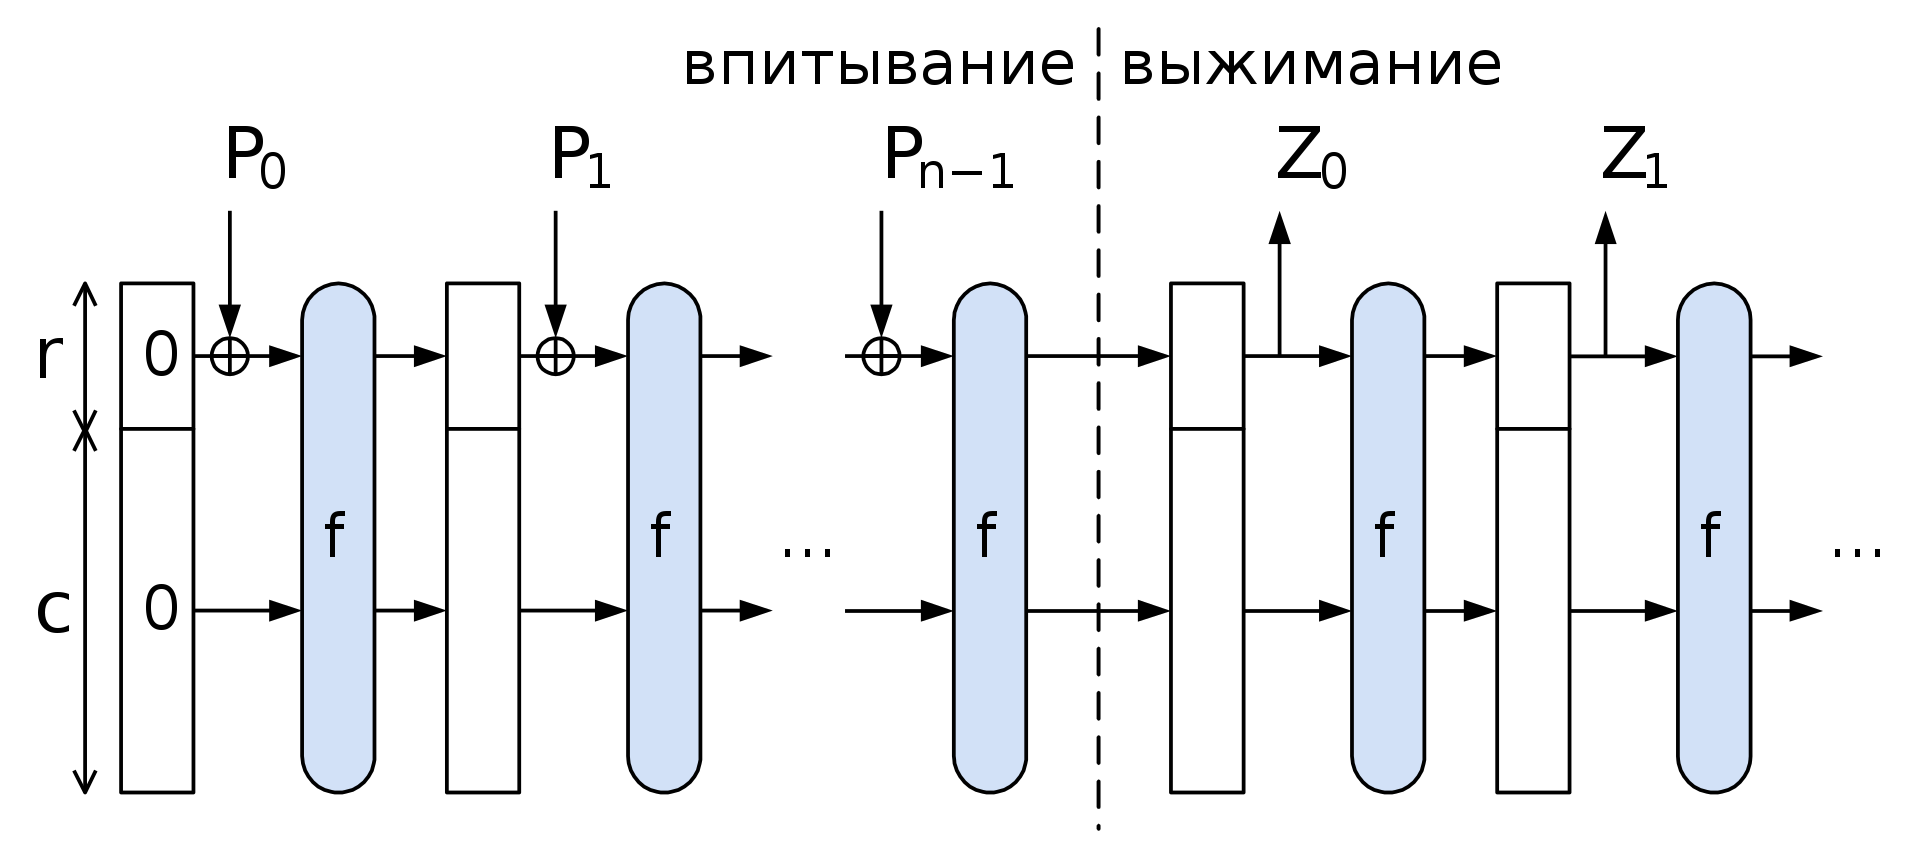
\includegraphics[width=0.5\linewidth]{SpongeConstruction.svg.png}
    \caption{Губка}
    \label{fig:enter-label}
\end{figure}

Функция губки (sponge function) - это одна из архитектур, которая используется для построения хеш-функций. Губка состоит из состояния $S$ (вектор битов) и функции псевдослучайной перестановки $f$. Состояние $S$ делится на 2 последовательные части: $c$ и $r$, которые состоят из $|c|$ и $|r|$ бит соответственно.

\textbf{Алгоритм работы}

На вход поступает сообщение $M$, которое разбивается на последовательные блоки длиной $|r|$. Затем эти блоки последовательно подаются в губку. Состояние $S$ инициализируется нулями.

\textit{Этап впитывания (absorbing).} На вход губке подается очередной блок текста длиной $|r|$. Он "ксорится" с частью $r$ состояния $S$, затем к $S$ применяется функция $f$. Затем подается следующий блок текста и аналогично обрабатывается, пока не закончатся блоки исходного сообщения.

Затем идет следующий этап. Определим желаемую длину выхода губки и создадим переменную $res$ этой длины, заполненную нулями.

\textit{Этап выжимания (squeezing).} Из $r$ (часть $S$) биты копируются $res$, затем к $S$ применяется $f$. Если переменная не заполнилась, то снова переносим данные из $r$ в $res$. Заметим, что переменная $res$ заполняется последовательно данными из $r$. По итогу в $res$ должна находится конкатенация данных из $r$, полученных на разных этапах. 

При необходимости можно взять, обрезанную часть $res$, если выход губки не кратен $r$.

\textbf{Особенности, достоинства, недостатки.}

Губка позволяет получить выход любой длины, задавая количество шагов в фазе выжимания. Также можно менять размер $c$ и $r$ состояния $S$. Увеличивая размер $c$, мы делаем выходную последовательность более устойчивой к криптоанализу и наоборот. Увеличивая размер $r$, мы увеличиваем скорость выдачи результирующих битов и наоборот. Поэтому важно найти баланс между стойкостью и "скоростью" губки. 

Если злоумышленник знает представление функции $f$ в виде циклов полностью или частично, то он способен строить коллизии для хеш-функции, в основе которой лежит губка [1].

\subsection{HAIFA}

Конструкция для хеш-функции HAIFA (HAsh Iterative FrAmework) является модификацией классической конструкции Меркла—Дамгарда.

\begin{figure}[H]
    \centering
    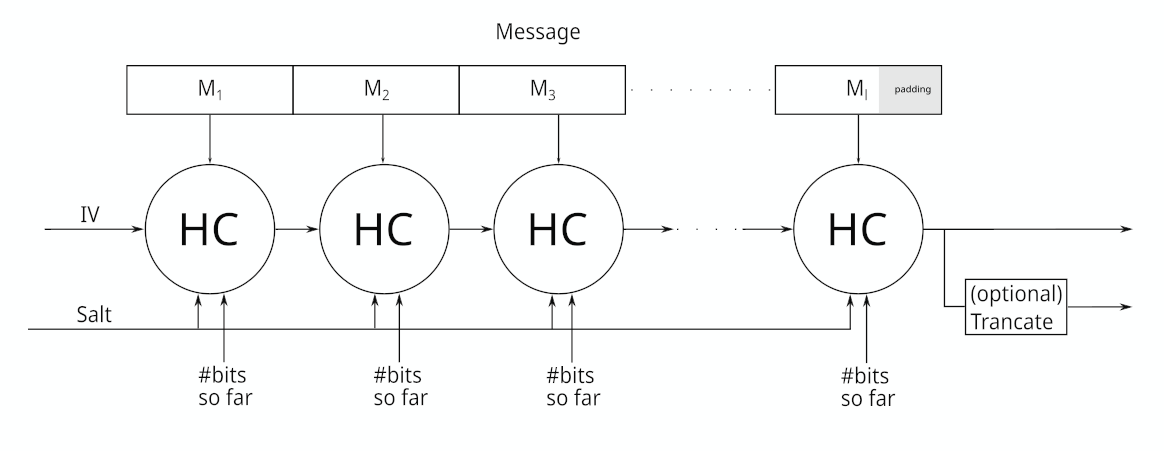
\includegraphics[width=0.75\linewidth]{kglcf.png}
    \caption{HAIFA}
    \label{fig:enter-label}
\end{figure}

\textbf{Алгоритм работы}

Перед хешированием сообщение дополняется следующими битами: одна единица, определенное количество нулей, длина сообщения в битах, длина хеша в битах. Нулей добавляется такое количество, которое сделает длину сообщения кратной длине блока.

На вход HAIFA подается сообщение $M$, инициализирующий вектор $IV$ и соль(salt):

\begin{enumerate}
    \item Сообщение $M$ дополняется и разбивается на блоки одинаковой длины $M_i$.
    \item $h_0 = IV$.
    \item Пока есть необработанный блок $M$, вычисляется функция $C: h_i = C(h_{i-1}, M_i, bits, salt)$.
    \item Финальное значение $h_i$ подается на выход.
\end{enumerate}

$bits$ на каждом этапе хеширования определяется количеством захешированных битов исходного сообщения к данному моменту.

\textbf{Особенности, достоинства, недостатки.}

Конструкция HAIFA устойчива к коллизиям, если функция $C$ устойчива к коллизиям. Соль пресекает атаки, которые используют предварительные вычисления. Функция $C$ является узким местом в данной конструкции, если не удается подобрать стойкую функцию, то HAIFA также не будет стойкой.

\section{MD5}

MD5(Message Digest 5) — алгоритм хеширования, разработанный в MIT в 1991 году. MD5 использует конструкцию Меркла-Дамгарда. В 1992 году алгоритм стал стандартом [2], опишем его.

\textbf{Функции и константы}

В MD5 используются следующие функции:

\begin{enumerate}
    \item $F(X, Y, Z)=(X \wedge Y) \vee(\neg X \wedge Z)$
    \item $G(X, Y, Z)=(X \wedge Z) \vee(\neg Z \wedge Y)$
    \item $H(X, Y, Z)=X \oplus Y \oplus Z$
    \item $I(X, Y, Z)=Y \oplus(\neg Z \vee X)$
\end{enumerate}

Также используется 64-элементный список 32-битных констант $T: T[n] = int(2^{32} * |sin(n)|), n = 1 \dots 64$.

\textbf{Алгоритм MD5}

У MD5 есть свое внутреннее 128-битное состояние, которое задается 32-битными словами A,B,C,D. Оно инициализируется следующим образом:

\begin{enumerate}
    \item $A = 0x 01 23 45 67$
    \item $B = 0x 89 ab cd ef$
    \item $C = 0x fe dc ba 98$
    \item $D = 0x 76 54 32 10$
\end{enumerate}

Входное сообщение $M$ дополняется единицей, нулями и длиной сообщения в битах (64 бита). Нулей добавляется такое количество, которое сделает длину сообщения кратной 512. Далее алгоритм по очереди обрабатывает 512-битные блоки.

Перед обработкой очередного блока 128-битное состояние запоминается, для простоты заведем переменную $res$, в которой будем хранить это состояние.

Обработка 512-битного блока проходит в 4 раунда, каждый раунд состоит из 16 итераций (блок делится на 16 32-битных частей и хранится в массиве $X$). После этого к текущему состоянию добавляется (операция "oplus") предыдущее состояние (оно у нас хранится в $res$).

Раунды выглядят следующим образом:

\begin{figure}[H]
    \centering
    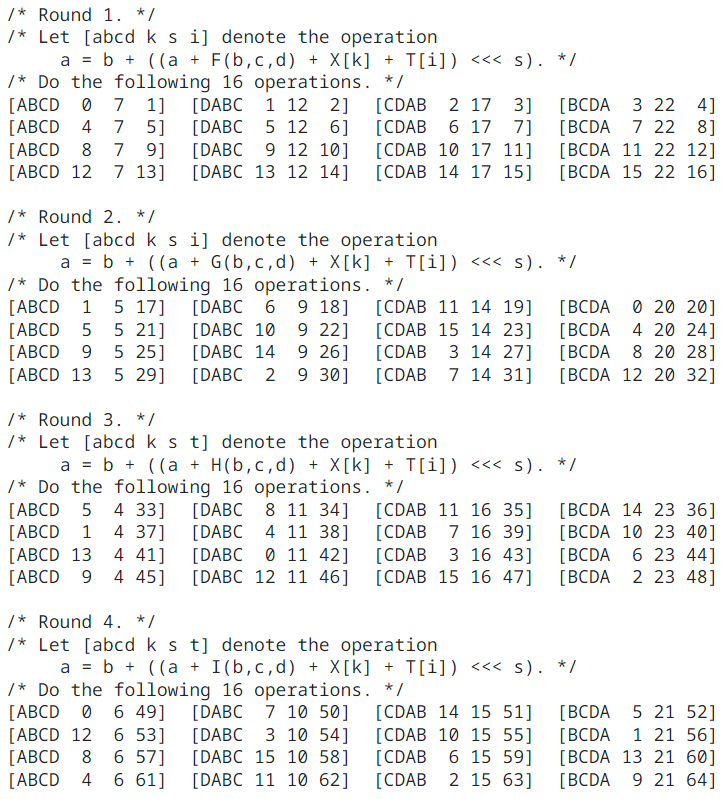
\includegraphics[width=0.5\linewidth]{md5.png}
    \caption{Раунды MD5}
    \label{fig:enter-label}
\end{figure}

Конечное 128-битное состояние является выходом MD5.


\section{SHA-1}

SHA-1 (Secure Hash Algorithm 1) — алгоритм хеширования, разработанный АНБ США в 1995 году [3]. Этот хеш также стал стандартом [4].

\textbf{Функции и константы}

В SHA-1 используются следующие функции и константы:

\begin{enumerate}
    \item $F_t(m, l, k)=(m \wedge l) \vee(\neg m \wedge k)$ , $K_t = 0x5A827999$, $0 \leq t \leq 19$
    \item $F_t(m, l, k)=m \oplus l \oplus k$ , $K_t = 0x6ED9EBA1$, $20 \leq t \leq 39$
    \item $F_t(m, l, k)=(m \wedge l) \vee(m \wedge k) \vee(l \wedge k)$ , $K_t = 0x8F1BBCDC$, $40 \leq t \leq 59$
    \item $F_t(m, l, k)=m \oplus l \oplus k$ , $K_t = 0xCA62C1D6$, $60 \leq t \leq 79$
\end{enumerate}

\textbf{Алгоритм SHA-1}

У SHA-1 есть свое внутреннее 160-битное состояние, которое задается 32-битными словами $H_0, H_1, H_2, H_3, H_4$. Оно инициализируется следующим образом:

\begin{enumerate}
    \item $H_0 = 0x67452301$
    \item $H_1 = 0xEFCDAB89$
    \item $H_2 = 0x98BADCFE$
    \item $H_3 = 0x10325476$
    \item $H_4 = 0xC3D2E1F0$
\end{enumerate}

Входное сообщение $M$ дополняется единицей, нулями и длиной сообщения в битах (64 бита). Нулей добавляется такое количество, которое сделает длину сообщения кратной 512. Далее алгоритм по очереди обрабатывает 512-битные блоки.

Обработка 512-битного блока проходит в несколько этапов:

\begin{enumerate}
    \item Блок состоит из 16 32-битных слов $W_t$. Блок расширяется до 80 32-битных слов по следующей формуле: $W_t = (W_{t-3} \oplus W_{t-8} \oplus W_{t-14} \oplus W_{t-16}) << 1$. 
    \item $A = H_0, B = H_1, C = H_2, D = H_3, E = H_4$
    \item Далее идет цикл по $t$: $0 \leq t \leq 79$ 
    
    \begin{itemize}
     \item $TEMP = (A << 5) + F_t(B,C,D) + E + W_t + K_t;$
     \item $E = D;  D = C;  C = (B << 30);  B = A; A = TEMP$
     \item $H_0 = H_0 + A, H_1 = H_1 + B, H_2 = H_2 + C, H_3 = H_3 + D, H_4 = H_4 + E$    
    \end{itemize}
    \item $H_0 += A, H_1 += B, H_2 += C, H_3 += D, H_4 += E$
\end{enumerate}

Операция $(A << n)$ означает циклический сдвиг $A$ влево на $n$ битов.

Конечное 160-битное состояние является выходом SHA-1.

\section{SHA-2 (только SHA-256)}
Семейство хеш-функции SHA-2 было разработано АНБ США и опубликовано NIST в 2002 году в стандарте FIPS PUB 180-2 [5].

\textbf{Константы}

В SHA-256 используются следующие константы:
\begin{figure}[H]
    \centering
    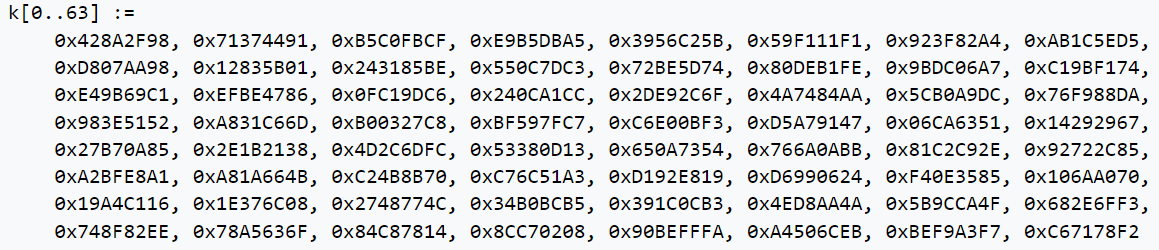
\includegraphics[width=0.6\linewidth]{sha_256_consts.png}
    \caption{Константы SHA-256}
    \label{fig:enter-label}
\end{figure}

\textbf{Алгоритм SHA-256}

У SHA-256 есть внутреннее 256-битное состояние, которое задается 32-битными словами $H_0, H_1, H_2, H_3, H_4, H_5, H_6, H_7$. 

Оно инициализируется следующим образом:

\begin{enumerate}
    \item $H_0 = 0x6A09E667$
    \item $H_1 = 0xBB67AE85$
    \item $H_2 = 0x3C6EF372$
    \item $H_3 = 0xA54FF53A$
    \item $H_4 = 0x510E527F$
    \item $H_5 = 0x9B05688C$
    \item $H_6 = 0x1F83D9AB$
    \item $H_7 = 0x5BE0CD19$
\end{enumerate}

Входное сообщение $M$ дополняется единицей, нулями и длиной сообщения в битах (64 бита). Нулей добавляется такое количество, которое сделает длину сообщения кратной 512. Далее алгоритм по очереди обрабатывает 512-битные блоки.

Обработка 512-битного блока проходит следующим образом:

\begin{enumerate}
    \item 512-битный блок разбивается на 16 32 битных слов: $w[0..15]$
    \item Генерация дополнительных 48 32-битных блоков:

    for $i$ := 16 to 63:

    \begin{aligned}
    & \text { so := (w[i-15] rotr } 7) \text { oplus }(w[i-15] \operatorname{rotr} 18) \text { oplus }(w[i-15] \text { shr } 3) \\
    & \text { s1 := (w[i-2] rotr } 17) \text { oplus }(w[i-2] \operatorname{rotr} 19) \text { oplus }(w[i-2] \text { shr } 10) \\
    & w[i]:=w[i-16]+s 0+w[i-7]+\text { s1 }
    \end{aligned}
    
    \item Инициализация временных переменных: $a := H_0, b := H_1, c := H_2, d := H_3, e := H_4, f := H_5, g := H_6, h := H_7$
    \item Основной цикл алгоритма.

    for $i$ := 0 to 63:

    \begin{itemize}
        \item $\Sigma0$:= (a rotr 2) oplus (a rotr 13) oplus (a rotr 22)
        \item $Ma$ := (a and b) oplus ( a and c) oplus (b and c)
        \item $t2 := \Sigma\theta + Ma$
        \item $\Sigma1$ := (e rotr 6) oplus (e rotr 11) oplus (e rotr 25)
        \item $Ch$ := (e and f) oplus ((not e) and g)
        \item $t1 := h + \Sigma1 + Ch + k[i] + w[i]$
        \item $h:=g$
        \item $g:=f$
        \item $f:=e$
        \item $e:=d+t1$
        \item $d:=c$
        \item $c:=b$
        \item $b:=a$
        \item $a := t1+t2$
    \end{itemize}
    
    \item Суммирования состояния с очередным результатом: $H_0$ += a, $H_1$ += b, $H_2$ += c, $H_3$ += d, $H_4$ += e, $H_5$ += f, $H_6$ += g, $H_7$ += h
\end{enumerate}

Примечание:

\begin{itemize}
        \item shr - логический сдвиг вправо.
        \item rotr — циклический сдвиг вправо.
\end{itemize}

Конечное 256-битное состояние является выходом SHA-256.

\section{SHA-3}
SHA-3 (Keccak) - алгоритм хеширования переменной разрядности, который построен с помощью архитектуры "губка". Этот алгоритм впервые был опубликован в 2008 году, в 2012 году он стал победителем конкурса от NIST и в 2015 - новым стандартом, оформленным в FIPS 202.

Так как SHA-3 основан на "губке", то для описания алгоритма достаточно описать параметры "губки", функцию паддинга и функцию перестановки $f$.

\textbf{Параметры "губки"}

Для SHA-3 длина внутреннего состояния равна 1600 бит. Количество раундов функции $f$ на один блок сообщения составляет 24. Длина выходного хеша может принимать значения :${224, 256, 384, 512}$. $r$ и $c$ принимают соответствующие значения:

\begin{figure}[H]
    \centering
    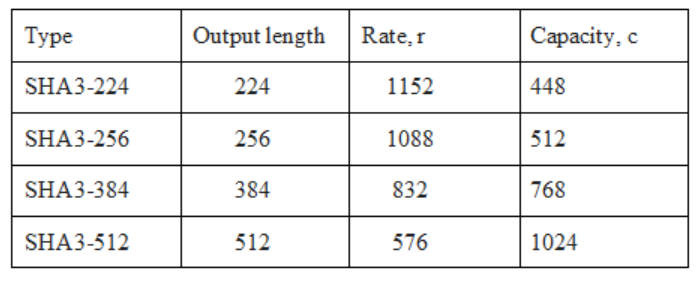
\includegraphics[width=0.6\linewidth]{sha3_rates.png}
    \caption{Таблица значений r, c для SHA-3}
    \label{fig:enter-label}
\end{figure}

\textbf{Функция паддинга}

Для алгоритма необходимо, чтобы в него подавались блоки сообщения размера $r$, поэтому каждое сообщение М необходимо дополнить битами справа, чтобы оно было кратно $r$.

\begin{itemize}
    \item Если |M| mod r = 0, то pad = "$10^{r-2}1$".
    \item Если |M| mod r = r-1, то pad = "$10^{r-1}1$".
    \item Иначе pad = "$10^{(r-2)-p}1$", где p = |M| mod r.
\end{itemize}

\textbf{Необходимые функции для SHA-3}

Состояние S отображается в трехмерный тензор $A$ размера 5*5*64 по формуле: $A[i][j][k] = S[(5i + j)*64+k]$, где $0<=i,j<=4$ и $0<=k<=63$. После отработки функции $f$ новый тензор $A'$ переводится в $S$ по той же формуле.

% $\theta, \rho, \pi, \chi, \iota$

Рассмотрим вспомогательную функцию $rc(t)$ и функции $\theta, \rho, \pi, \chi, \iota$:

\textit{Функция $rc(t)$}

На вход она получает целое число $t$.

\begin{enumerate}
    \item Если t mod 255 = 0, то return 1.
    \item Обозначим R = $[10000000]$.
    \item for i = 1 to (t mod 255):

        \begin{enumerate}
            \item R = 0 || R
            \item R[0] = R[0] $\oplus$ R[8]
            \item R[4] = R[4] $\oplus$ R[8]
            \item R[5] = R[0] $\oplus$ R[8]
            \item R[6] = R[0] $\oplus$ R[8]
            \item R = R[:8] (обрезаем крайний элемент)
        \end{enumerate}
        
    \item Возвращаем R[0].
\end{enumerate}

Далее везде, где не указано специально итерация по индексам будет проходить в этом диапазоне: $0<=i,j<=4$ и $0<=k<=63$

\textit{Функция $\theta(A)$}

Для всех (i, k):

\begin{aligned}
    & C(i, k)=A[i, 0, k] \oplus A[i, 1, k] \oplus A[i, 2, k] \oplus A[i, 3, k] \oplus A[i, 4, k] \\
    & D(i, k)=C[(i-1) \bmod 5, k] \oplus C[(i+1) \bmod 5,(k-1) \bmod w]
\end{aligned}

Для всех (i, j, k): $A[i,j,k] = A[i,j,k] + D[i, k]$

\textit{Функция $\rho(A)$}

Пусть (i, j) = (1, 0). Для t от 0 до 23:

\begin{enumerate}
    \item Для всех k: $A[i, j , k] = A[i, j , (k - (t+1)(t+2)/2) mod 64]$
    \item (i, j) = (j, (2i+3j) mod 5)
\end{enumerate}

\textit{Функция $\pi(A)$}

Для всех (i, j, k): $A[i,j,k] = A[(i+3j) mod 5, i, k]$


\textit{Функция $\chi(A)$}

Для всех (i, j, k): $A[i,j,k] = A[i,j,k] \oplus ((A[(i+1) mod 5, j, k] \oplus 1) * A[(i+2) mod 5, j, k])$

\textit{Функция $\iota(A, i_r)$}

\begin{enumerate}
    \item Пусть RC нулевой массив длины 64.
    \item Для i от 0 до 6: RC[$2^i-1$] = rc($i+7*i_r$).
    \item Для всех k: $A[0,0,k] = A[0,0,k] \oplus RC[k]$
\end{enumerate}

\textit{Функция перестановки $f(S)$}

% $\theta, \rho, \pi, \chi, \iota$

\begin{enumerate}
    \item Перевод состояния S в тензор A.
    \item Для $i_r$ от 0 до 23: $A = \iota(\chi(\pi(\rho(\theta(A)))), i_r)$.
    \item Перевод тензора A в состояние S.
\end{enumerate}

\section{ГОСТ Р 34.11-94}
ГОСТ Р 34.11-94 «Информационная технология. Криптографическая защита информации. Функция хэширования» - российский стандарт криптографической хеш-функции, который приняли в 1994 году. В 2013 году его отменили в РФ.

% \textbf{Алгоритм ГОСТ Р 34.11-94}

Эта хеш-функция основана на конструкции Меркла-Дамгарда с функцией сжатия $f$, которая принимает 2 блока по 256 бит и выдает блок длиной 256 бит. Рассмотрим функцию паддинга и функцию сжатия $f$.

\begin{figure}[H]
    \centering
    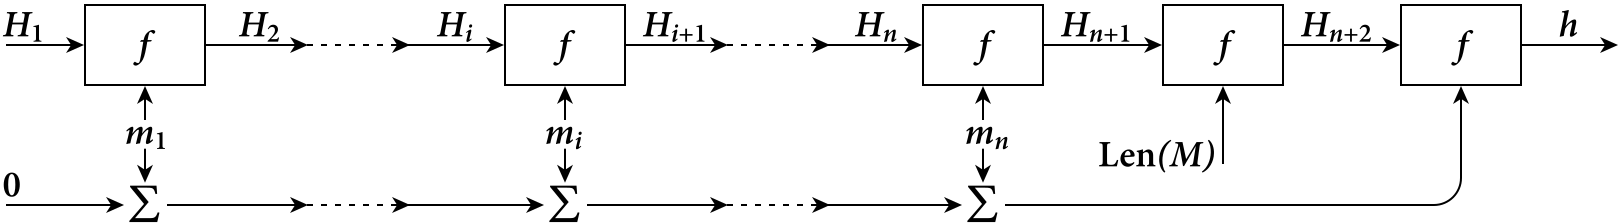
\includegraphics[width=0.75\linewidth]{GOST-hash-calculation.svg.png}
    \caption{Cхема хеш-функции ГОСТ Р 34.11-94}
    \label{fig:enter-label}
\end{figure}

\textbf{Функция паддинга}

Входное сообщение $M$ делится на блоки по 256 бит, если крайний блок не кратен 256 бит, то он \textbf{слева} дополняется нулями так, чтобы длина блока была 256 бит. Затем добавляется блок в 256 бит, кодирующий изначальную длину сообщения. И еще добавляется блок, который является суммой по модулю 2 всех 256-битных блоков исходного сообщения.

\textbf{Функция сжатия $f$}

Функции сжатия $f(H_{i-1}, m) = H_i$ принимает 2 блока длиной 256 бит и выдает один блок длиной 256 бит. Эта функция состоит из трех частей: генерация ключей, шифрующее преобразование, перемешивание.

\textit{Генерация ключей}

На этом этапе генерируется 4 ключа: $K_1, K_2, K_3 и K_4$.

Пусть есть 256-битный блок $Y=y_4||y_3||y_2||y_1$ или $Y=y_{32}||y_{31}||...||y_1$. Для генерации используется 2 функции, которые преобразуют 256-битный блок:

\begin{itemize}
    \item $A(Y) = (y_1 \oplus y_2)||y_4||y_3||y_2$
    \item $P(Y) = y_{\phi(32)}||y_{\phi(31)}||...||y_{\phi(31)}$, где $\phi(i+1+4(k-1)) = 8i+k$ при $i=0,...,3$, $k=1,...,8$ 
\end{itemize}

Также используются константы: 

\begin{itemize}
    \item $C_2, C_4 = 0$
    \item $C_3 = 0xff00ffff000000ffff0000ff00ffff0000ff00ff00ff00ffff00ff00ff00ff00$
\end{itemize}

Алгоритм генерации ключей:

\begin{enumerate}
    \item $U := H_{in}, \quad V := m, \quad W := U \oplus V, \quad K_1 = P(W)$
    \item Для j от 2 до 4:

    $U:=A(U) \oplus C_j, \quad V:=A(A(V)), \quad W:=U \oplus V, \quad K_j=P(W)$
\end{enumerate}

\textit{Шифрующее преобразование}

На этом этапе происходит шифрование $H_{in}=h_4||h_3||h_2||h_1$ с помощью сгенерированных ключей $K_1, K_2, K_3, K_4$. Шифрование происходит с помощью блочного шифра ГОСТ 28147—89 $E$ [6]: $s_i = E(h_i, K_i)$, для i от 1 до 4. Выходом этого преобразования является: $S=s_4||s_3||s_2||s_1$

\textit{Перемешивание}

На этом этапе 256-битный блок $S$ и 256-битный блок сообщения $m$ перемешиваются с помощью регистра сдвига с линейной обратной связью. РСЛОС определяется как $\psi(Y=y_{16}||y_{15}||...||y_1)=(y_1 \oplus y_2 \oplus y_3 \oplus y_4 \oplus y_{13} \oplus y_{16})||y_{16}||y_{15}||...||y_{2}$. В итоге перемешивающее образование имеет вид:

$H_{out} = \psi^{61}(H_{in} \oplus \psi(m \oplus \psi^{12}(S)))$


\section{ГОСТ 34.11-2018 (Стрибог)}
ГОСТ 34.11-2018 (Стрибог) «Информационная технология. Криптографическая защита информации. Функция хэширования» - межгосударственный криптографический стандарт хеш-функции, который приняли в 2018 году. В его основе лежит ГОСТ Р 34.11-2012, который в свою очередь пришел на смену устаревшему ГОСТ Р 34.11-94. Он может выдавать хеш размером 256 или 512 бит, рассмотрим 512-битный вариант.

Эта хеш-функция основана на конструкции Меркла-Дамгарда с функцией сжатия $g$, которая принимает 3 блока по 512 бит и выдает блок длиной 512 бит. Также $H_0 = IV = 0^{512}$. Рассмотрим функцию паддинга и функцию сжатия $g$.

\begin{figure}[H]
    \centering
    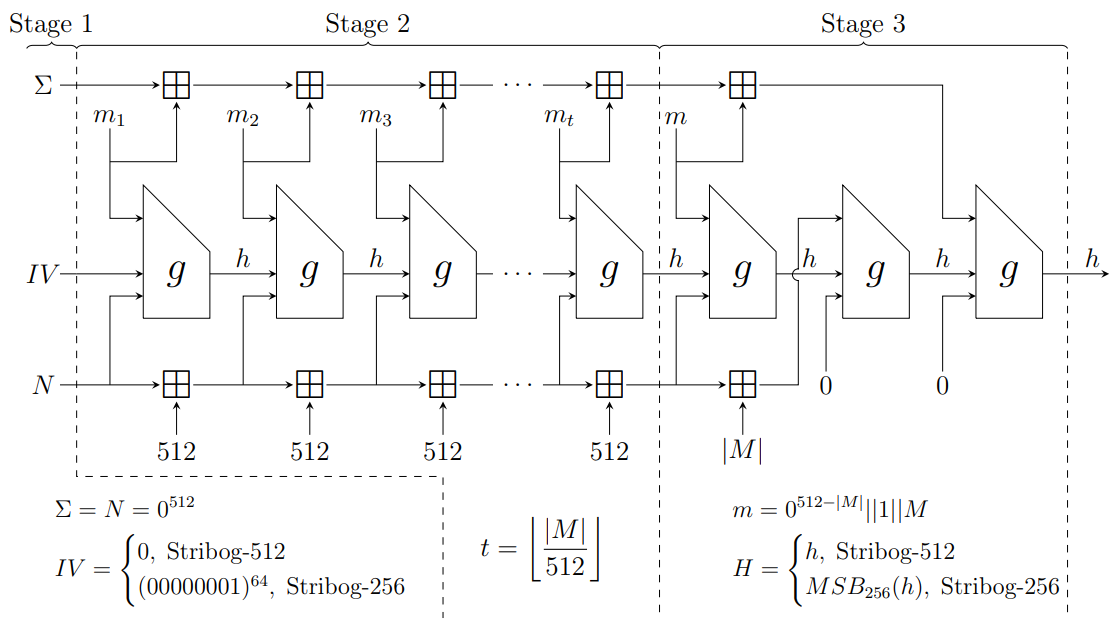
\includegraphics[width=0.75\linewidth]{gost_34_11_2018.png}
    \caption{Схема хеш-функции ГОСТ 34.11-2018 (Стрибог) [7]}
    \label{fig:enter-label}
\end{figure}

\textbf{Функция паддинга}

Входное сообщение $M$ делится на блоки по 512 бит, если крайний блок не кратен 512 бит, то он \textbf{слева} дополняется нулями и одной единицей ($0^*1$) так, чтобы длина блока была 512 бит. Затем добавляется блок в 512 бит, кодирующий изначальную длину сообщения. И еще добавляется блок, который является суммой по модулю 2 всех 512-битных блоков исходного сообщения.

\textbf{Функция сжатия $g$}

В ГОСТ 34.11-2018 функция сжатия $g$ основана на конструкции Миагути - Пренеля. На вход она принимает $N$ (сумма обработанных на текущий момент битов исходного сообщения в 512-битном представлении, для двух последних блоков $N=0$) и 2 512-битных блока $h$ и $m$. Рассмотрим $g_N(h, m)$:

\begin{figure}[H]
    \centering
    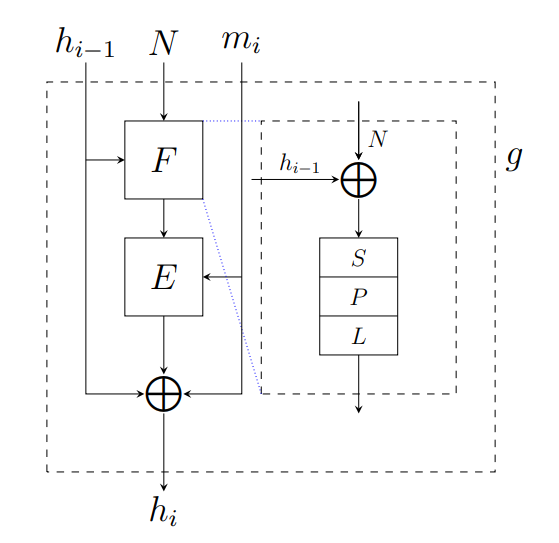
\includegraphics[width=0.5\linewidth]{streebog_F.png}
    \caption{Схема функции сжатия g в ГОСТ 34.11-2018 [7]}
    \label{fig:enter-label}
\end{figure}

\begin{enumerate}
    \item $g_N(h, m)=E(L \circ P \circ S(h \oplus N), m) \oplus h \oplus m$
    \item $E(K, m)=X\left[K_{13}\right] \circ \prod_{i=1}^{12}\left(L \circ P \circ S \circ X\left[K_i\right](m)\right)$
    \item $K_i=L \circ P \circ S\left(K_{i-1} \oplus C_{i-1}\right), K_1=K, i \in\{2, \ldots, 13\}$. Константы $C_i$ можно найти в стандарте [8].
    \item $X[K_i](A)$ = $A \oplus K_i$
    \item S (SubBytes) нелинейно преобразует каждые 8 бит в другие 8 бит с помощью перестановки (ее можно найти в стандарте [8]).
    \item P (Permutation) это перестановка байт в 512 блоке (ее можно найти в стандарте [8]).
    \item L (MixColumns)  это линейное преобразование, при котором 512-битный блок представляется в виде матрицы размер 64x64 и умножается справа на специальную матрицу, операции проводятся по модулю 2 (ее можно найти в стандарте [8]).
\end{enumerate}

Выходом алгоритма является крайнее значение $h$.

\section{BLAKE-256}
BLAKE - криптографическая хеш-функция [10], основанная на конструкции HAIFA и использующий идеи потокового шифра ChaCha. Эта функция оказалась финалистом конкурса NIST на SHA-3, уступив алгоритму Keccak в 1012 году. Существуют версии с выходом в 224, 256, 384 или 512 бит. Рассмотрим версию с 256-битным выходом BLAKE-256.

\begin{figure}[H]
    \centering
    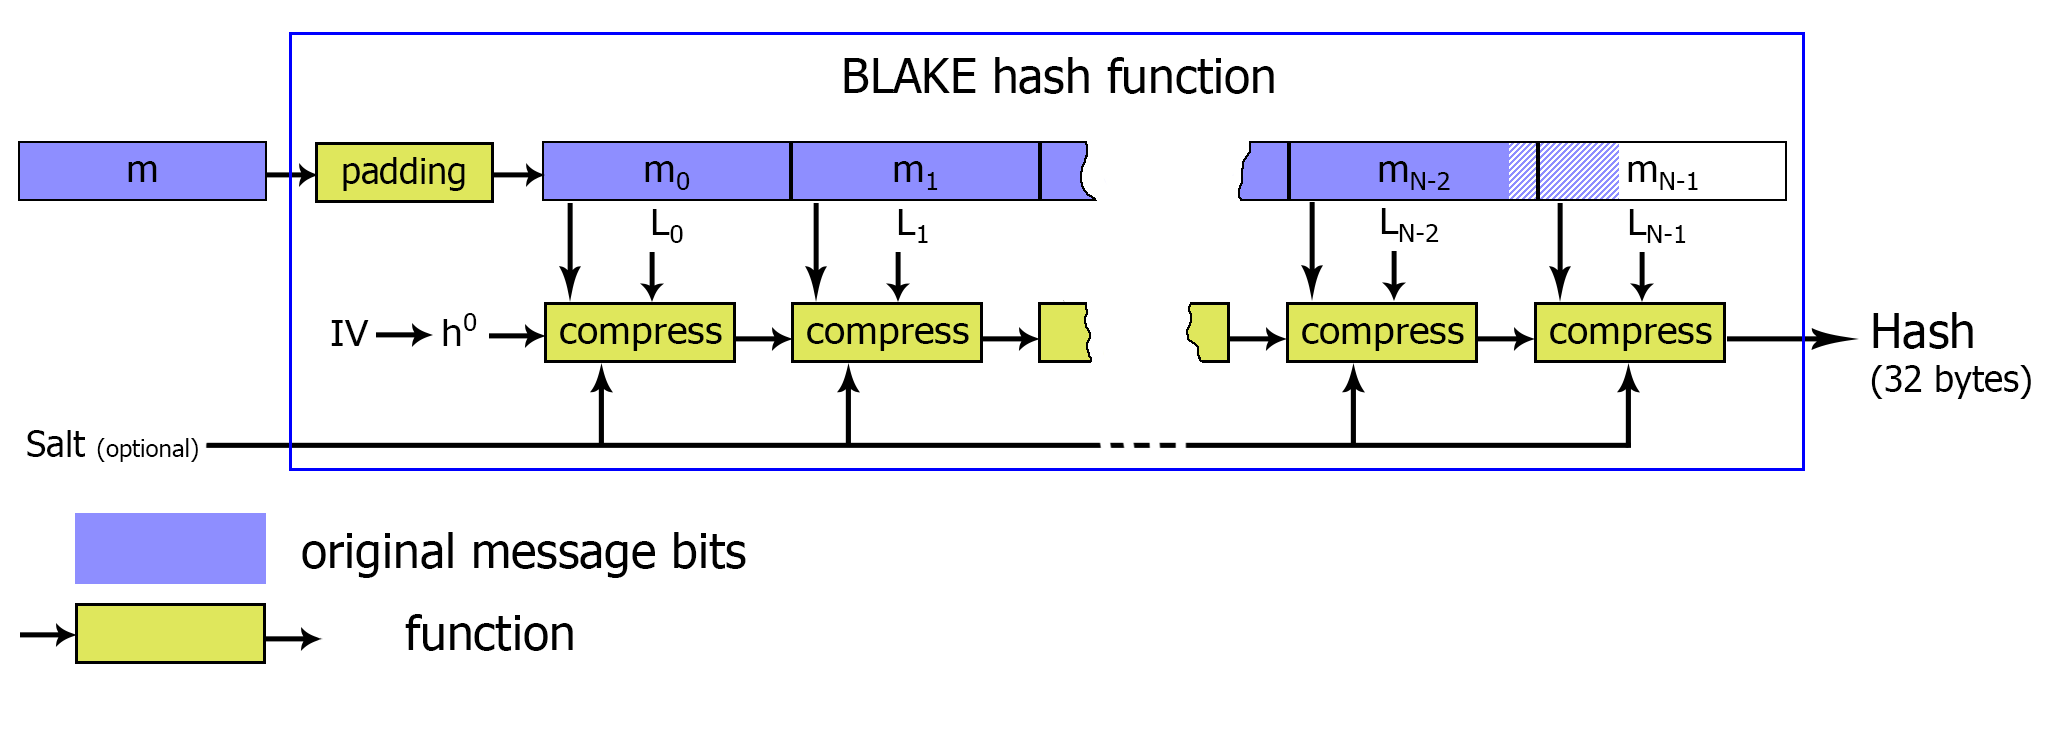
\includegraphics[width=0.75\linewidth]{BLAKE_algorythm.png}
    \caption{Схема BLAKE-256 [9]}
    \label{fig:enter-label}
\end{figure}

\textbf{Константы и перестановки}

В BLAKE-256 используются следующие константы:

\begin{figure}[H]
    \centering
    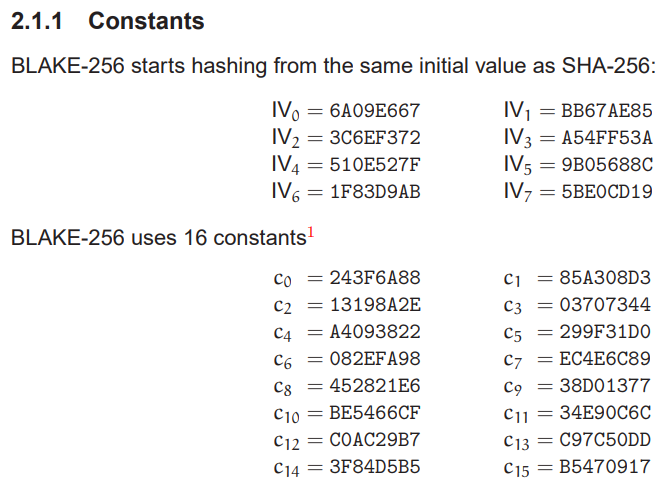
\includegraphics[width=0.5\linewidth]{constants_blake.png}
    \caption{Константы хеш-функции BLAKE-256 [10]}
    \label{fig:enter-label}
\end{figure}

В BLAKE-256 используются следующие перестановки:

\begin{figure}[H]
    \centering
    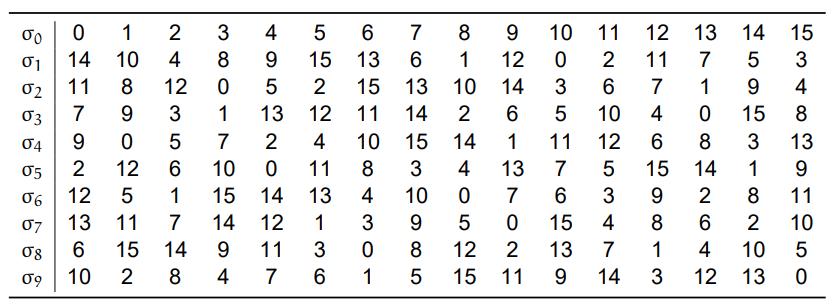
\includegraphics[width=0.5\linewidth]{permutations_blake.png}
    \caption{Перестановки $S_16$ хеш-функции BLAKE-256 [10]}
    \label{fig:enter-label}
\end{figure}

\textbf{Функция паддинга}

BLAKE обрабатывает 512-битные блоки сообщения, поэтому необходимо добавить справа столько бит, чтобы длина сообщения стала кратна 512. Справа добавляется следующие биты: $pad=10^*1L_{64}$, где $L_{64}$ - это длина исходного сообщения в 64-битном представлении.

\textbf{Функция сжатия $compress$}

Функция сжатия $compress$ принимает на вход 4 параметра:

\begin{itemize}
    \item 256-битное состояние $h=h_0||...||h_7$
    \item 512-битный блок сообщения $m=m_0||...||m_{15}$
    \item 128-битный блок соли $s=s_0||...||s_3$
    \item 64-битный блок счетчика $t=t_0||t_1$
\end{itemize}

\textit{Этап инициализации}. Начинается инициализация внутренних 32-битных переменных $v_0, \ldots, v_{15}$:

$\newline$

$\left(\begin{array}{cccc}
v_0 & v_1 & v_2 & v_3 \\
v_4 & v_5 & v_6 & v_7 \\
v_8 & v_9 & v_{10} & v_{11} \\
v_{12} & v_{13} & v_{14} & v_{15}
\end{array}\right) \leftarrow\left(\begin{array}{cccc}
h_0 & h_1 & h_2 & h_3 \\
h_4 & h_5 & h_6 & h_7 \\
s_0 \oplus c_0 & s_1 \oplus c_1 & s_2 \oplus c_2 & s_3 \oplus c_3 \\
t_0 \oplus c_4 & t_0 \oplus c_5 & t_1 \oplus c_6 & t_1 \oplus c_7
\end{array}\right)$

$\newline$

\textit{Этап основной работы}. Затем идет 14 раундов работы алгоритма над внутренними переменными. Один раунд выглядит так:

$\newline$

$\begin{aligned}
& G_\theta\left(v_0, v_4, v_8, v_{12}\right) G_1\left(v_1, v_5, v_9, v_{13}\right) G_2\left(v_2, v_6, v_{10}, v_{14}\right) G_3\left(v_3, v_7, v_{11}, v_{15}\right) \\
& G_4\left(v_0, v_5, v_{10}, v_{15}\right) G_5\left(v_1, v_6, v_{11}, v_{12}\right) G_6\left(v_2, v_7, v_8, v_{13}\right) G_7\left(v_3, v_4, v_9, v_{14}\right)
\end{aligned}$

$\newline$

$G_i(a,b,c,d)$ работает так:

$\newline$

$\begin{aligned}
& j \leftarrow \sigma_{r \% 10}[2 \times i] \\
& k \leftarrow \sigma_{r \% 10}[2 \times i+1] \\
& a \leftarrow a+b+\left(m_j \oplus c_k\right) \\
& d \leftarrow(d \oplus a)>>>16 \\
& c \leftarrow c+d \\
& b \leftarrow(b \oplus c)>>>12 \\
& a \leftarrow a+b+\left(m_k \oplus c_j\right) \\
& d \leftarrow(d \oplus a)>>>8 \\
& c \leftarrow c+d \\
& b \leftarrow(b \oplus c)>>>7
\end{aligned}$

$\newline$

\textit{Финальный этап}. В конце подсчитывается выходное значение функции сжатия из внутренних переменных, соли и предыдущего выходного значения:

$\newline$

$\begin{aligned}
& \mathrm{h}_0^{\prime} \leftarrow \mathrm{h}_0 \oplus \mathrm{s}_0 \oplus v_0 \oplus v_8 \\
& \mathrm{~h}_1^{\prime} \leftarrow \mathrm{h}_1 \oplus \mathrm{s}_1 \oplus v_1 \oplus v_9 \\
& \mathrm{~h}_2^{\prime} \leftarrow \mathrm{h}_2 \oplus \mathrm{s}_2 \oplus v_2 \oplus v_{10} \\
& \mathrm{~h}_3^{\prime} \leftarrow \mathrm{h}_3 \oplus \mathrm{s}_3 \oplus v_3 \oplus v_{11} \\
& \mathrm{~h}_4^{\prime} \leftarrow \mathrm{h}_4 \oplus \mathrm{s}_0 \oplus v_4 \oplus v_{12} \\
& \mathrm{~h}_5^{\prime} \leftarrow \mathrm{h}_5 \oplus \mathrm{s}_1 \oplus v_5 \oplus v_{13} \\
& \mathrm{~h}_6^{\prime} \leftarrow \mathrm{h}_6 \oplus \mathrm{s}_2 \oplus v_6 \oplus v_{14} \\
& \mathrm{~h}_7^{\prime} \leftarrow \mathrm{h}_7 \oplus \mathrm{s}_3 \oplus v_7 \oplus v_{15}
\end{aligned}$

$\newline$

Таким образом, на выход идет 256-битный блок $h_{0}^{'}||...||h_{7}^{'}$.

\section{RIPEMD-256}

RIPEMD-256 - криптографическая хеш-функция, по факту состоящая из двух копий RIPEMD-128 и соответственно имеющая такой же уровень безопасности как RIPEMD-128. RIPEMD-128 была разработана в 1996 году.

RIPEMD-128 - криптографическая хеш-функция, построенная на конструкции Меркла-Дамгарда и имеющая 128-битный выход.

\textbf{Функция паддинга}

RIPEMD-128 работает с 512-битными блоками сообщения, поэтому нужно сделать длину сообщения кратной 512. Справа к сообщению добавляется единица, нули и длина сообщения, закодированная в 64-битном блоке. Нулей добавляется столько, чтобы длина сообщения стала кратна 512.

\textbf{Необходимые константы и функции}

Обозначим необходимые константы и функции для работы RIPEMD-128:

\begin{figure}[H]
    \centering
    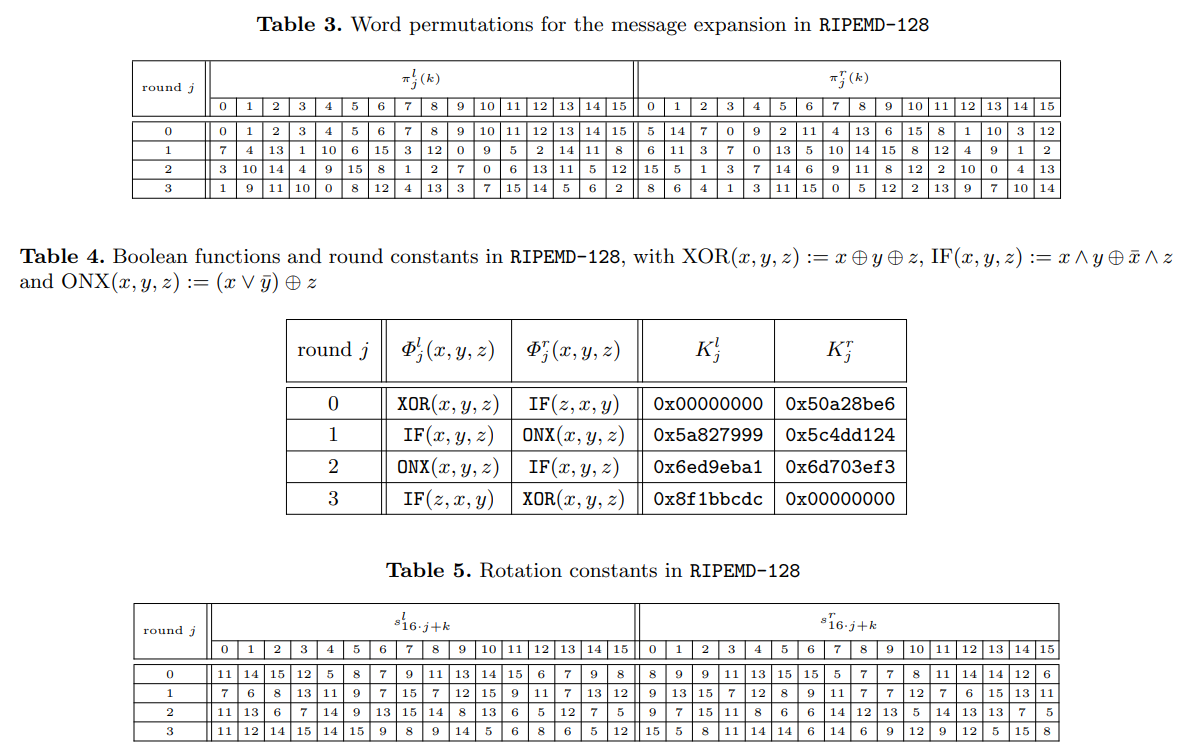
\includegraphics[width=0.75\linewidth]{ridemp_consts.png}
    \caption{Таблица функции и констант, необходимых для RIPEMD-128}
    \label{fig:enter-label}
\end{figure}

\textbf{Функция сжатия $f$}

Функция сжатия $f(h, m)$ принимает на вход 128-битный блок $h=h_0||h_1||h_2||h_3$ и 512-битный блок сообщения $m$. 

\textit{Этап инициализации}. RIPEMD-128 имеет внутреннее 256-битное состояние, состоящее из двух так называемых ветвей: левой ветви $X$ и правой ветви $Y$. Они инициализируются следующим образом:

$\begin{array}{llll}
X_{-3}=h_0 & X_{-2}=h_1 & X_{-1}=h_2 & X_0=h_3 \\
Y_{-3}=h_0 & Y_{-2}=h_1 & Y_{-1}=h_2 & Y_0=h_3
\end{array}$

Если это самая первая итерация функции сжатия, то ветви инициализируются так:

$X_{-3}=Y_{-3}=0 \mathrm{x} 67452301 \quad X_{-2}=Y_{-2}=\text { 0xefcdab89 } \quad X_{-1}=Y_{-1}=0 \mathrm{x} 98 \mathrm{badcfe} \quad X_0=Y_0=0 \times 10325476$

\textit{Этап расширения блока сообщения}. Входной блок сообщения $m=m_0||...||m_15$ представляется в виде 16 32-битных слов. Заводится 2 массива длиной 64 элемента: $W^l$ и $W^r$. Они заполняются следующим образом. Для всех (j, k): $0<=j<=3$, $0<=k<=15$:

\begin{itemize}
    \item $W_{j \cdot 16+k}^l=M_{\pi_j^l(k)}$
    \item $W_{j \cdot 16+k}^r=M_{\pi_j^r(k)}$
\end{itemize}

\textit{Основной этап}. Далее идет 64 шага, разделенных на 4 раунда по 16 шагов. 1 шаг выглядит так:

$\begin{aligned}
X_{i+1} & =\left(X_{i-3} \boxplus \Phi_j^l\left(X_i, X_{i-1}, X_{i-2}\right) \boxplus W_i^l \boxplus K_j^l\right)^{\ll  s_i^l} \\
Y_{i+1} & =\left(Y_{i-3} \boxplus \Phi_j^r\left(Y_i, Y_{i-1}, Y_{i-2}\right) \boxplus W_i^r \boxplus K_j^r\right)^{\ll s_i^r}
\end{aligned}$

Где $i$ - номер шага ($o<=i<=63$), а $j$ - номер раунда ($o<=j<=3$), $\ll k$ - циклический сдвиг влево на k.

\textit{Финальный этап}. Выход функции сжатия $h^{'}=h^{'}_{0}||\ldots||h^{'}_{3}$ считается по следующей формуле:

$\begin{array}{ll}
h_0^{\prime}=X_{63} \boxplus Y_{62} \boxplus h_1 & h_1^{\prime}=X_{62} \boxplus Y_{61} \boxplus h_2 \\
h_2^{\prime}=X_{61} \boxplus Y_{64} \boxplus h_3 & h_3^{\prime}=X_{64} \boxplus Y_{63} \boxplus h_0
\end{array}$

\section{Whirlpool}
Whirlpool — криптографическая хеш-функция, первая версия которой появилась в 2000 году. Рассмотрим последнюю версию [11], которая вошла в стандарт ISO/IEC 10118-3:2004.

Whirlpool основана на конструкции Меркла-Дамгарда, функция сжатия основана на конструкции Миагути - Пренеля. Функция сжатия принимает 2 блока по 512-бит и выдает один 512-битный блок.

\textbf{Функция паддинга}

Необходимо, чтобы длина $M$ была кратна 512. Для этого перед вычислением хеша сообщение обрабатывается следующим образом:

\begin{itemize}
    \item К концу сообщения справа добавить единицу.
    \item Затем добавить такое количество нулей справа, чтобы итоговая длина сообщения была нечетное количество раз кратна 256.
    \item Добавить справа 256-битное представление длины исходного сообщения.
\end{itemize}

\textbf{Алгоритм Whirlpool}

После выравнивания сообщения $M$ оно разбивается на $t$ блоков по 512-бит $m_i$, которые по очереди обрабатываются по следующему алгоритму:

$\newline$

$\begin{aligned}
\eta_i & =\mu\left(m_i\right) \\
H_0 & =\mu(I V) \\
H_i & =W\left[H_{i-1}\right]\left(\eta_i\right) \oplus H_{i-1} \oplus \eta_i, 1 \leqslant i \leqslant t
\end{aligned}$

Здесь $IV=0^{512}$. Выходом хеш-функции является 512-битный блок $H_t$.

Рассмотрим функции $\mu$ и блочный шифр $W$:

$\newline$

\textit{Функция $\mu$}

Функция $\mu(a)$ на вход принимает 512-битный вектор $a$ и возвращает матрицу размера 8*8 внутри которой расположены байты. Преобразование происходит по следующей формуле:

$\mu(a)=b \Leftrightarrow b_{i j}=a_{8 i+j}, 0 \leqslant i, j \leqslant 7$

Индексация в $a$ происходит побайтово.

$\newline$

\textit{Вычисление ключей}

Из ключа $K$, который является матрицей 8*8 вычисляются ключи по следующей формуле:

$\begin{aligned}
& K^0=K \\
& K^r=\rho\left[c^r\right]\left(K^{r-1}\right), r>0
\end{aligned}$

$\newline$

\textit{Функция $\gamma$}

Эта функция нелинейно преобразует каждый байт входной матрицы с помощью специального S-box'a, который описан в [11]:

$\gamma(a)=b \Leftrightarrow b_{i j}=S[a_{ij}], 0 \leqslant i, j \leqslant 7$


$\newline$

\textit{Функция $\pi$}

Функция циклической перестановки $\pi$, которая задается следующим образом:

$\pi(a)=b \Leftrightarrow b_{i j}=a_{(i-j) \quad mod \quad 8, j}, 0 \leqslant i, j \leqslant 7$


$\newline$

\textit{Функция $\theta$}

Функция линейной диффузии $\theta$, которая входную матрицу умножает справа на специальную матрицу (все операции проходят по модулю 256):

$\theta(a)=b \Leftrightarrow b=a * C$

Матрица $C$ выглядит так:

\begin{figure}[H]
    \centering
    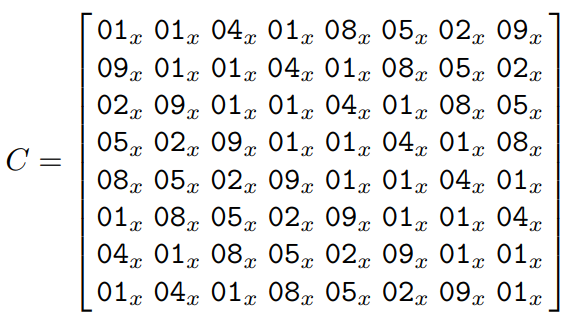
\includegraphics[width=0.5\linewidth]{whirlpool_matrix.png}
    \caption{Матрица $C$ хеш-фукнции Whirlpool [11]}
    \label{fig:enter-label}
\end{figure}

$\newline$

\textit{Функция $\sigma$}

Функция $\sigma$ подмешивает ключ к входному аргументу:

$\sigma[k](a)=b \Leftrightarrow b_{i j}=a_{ij} \oplus k_{ij}, 0 \leqslant i, j \leqslant 7$

$\newline$

\textit{Раундовые константы $c^r$}

Раундовые константы $c^r$ задаются следующим образом:

$\begin{array}{ll}
c_{0 j}^r \equiv S[8(r-1)+j], & 0 \leqslant j \leqslant 7 \\
c_{i j}^r \equiv 0, & 1 \leqslant i \leqslant 7,0 \leqslant j \leqslant 7
\end{array}$

$\newline$

\textit{Функция $\rho[K]$}

Функция $\rho[K]$ задается следующим образом:

$\rho[k] \equiv \sigma[k] \circ \theta \circ \pi \circ \gamma$

$\newline$

\textit{Блочный шифр $W[]()$}

Блочный шифр $W[K](\eta)$ задается как параметризованная функция от $K$, которая преобразует входную матрицу размера 8*8 в выходную матрицу размера 8*8. Задается она следующим образом:

$\newline$

$W[K]=({\bigcirc_1^{r=R}} \rho\left[K^r\right]) \circ \sigma\left[K^0\right]$ (композиция из 11 функций)

Ключи $K_i$ вычисляются из $K$. Дефолтное количество раундов $R=10$.

\subsection{Криптоанализ. Rebound attack}

В течении 8 лет c момента ее появления на эту хеш-функцию не было представлено ни одной атаки. И вот в 2009 году была опубликована первая атака нового типа - Rebound attack [13].

\textbf{Rebound attack}

Переобозначим функции в хеш-функции: 

\begin{itemize}
    \item $\sigma$ = AK
    \item $\theta$ = SB
    \item $\pi$ = SC
    \item $\gamma$ = MR
    \item Соответственно  раунд Whirlpool представляется как: $r := AK \circ MR \circ SC \circ SB$.
\end{itemize}

\begin{figure}[H]
    \centering
    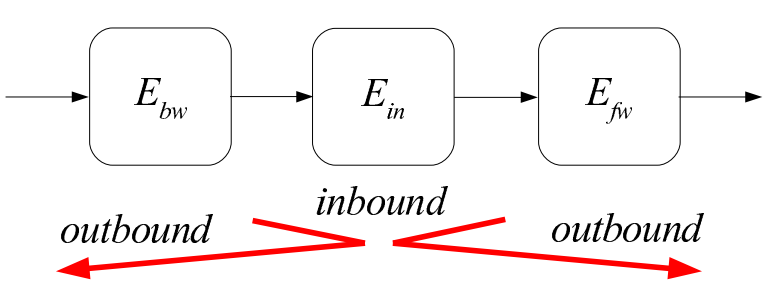
\includegraphics[width=0.5\linewidth]{rebound.png}
    \caption{Общая схема Rebound attack [13]}
    \label{fig:enter-label}
\end{figure}

Атака делится на два концептуальных этапа:

\begin{enumerate}
    \item \textbf{Inbound phase}: Фаза "встречи посередине" $E_{in}$, в котором есть достаточно пространство для подбора переменных для нахождения "встречи"(match).
    \item \textbf{Outbound phase}: В этой фазе используются усеченные дифференциалы, который как раз находятся в первой фазе, и распространяются вперед и назад в сторону $E_{fw}$ и $E_{bw}$ Соответственно . Если усеченные дифференциалы имеют низкую вероятность, тогда необходимо увеличить количество итерации в первой фазе, чтобы их найти. Таким образом находится вероятный дифференциал между входом и выходом алгоритма, с помощью которого строится коллизия, полусвободная коллизия или полусвободная почти коллизия.
\end{enumerate}

Авторы описали 3 атаки: на 4.5, 5.5 и 7.5 раундов. Рассмотрим атаку на 4.5 раундов.

Основная идея атаки - это найти последовательность дифференциалов, которая проходит через несколько активных S-box'ов: (1, 8, 64, 8, 1) S-box'ов Соответственно. Начало последовательности совпадает со входом в хеш-функцию и конец с концом 4.5 раунда. $E_{bw}, E_{in}, E_{fw}$ определяются следующим образом:

\begin{itemize}
    \item $E_{bw} = SC \circ SB \circ AK \circ MR \circ SC \circ SB$
    \item $E_{in} = MR \circ SC \circ SB \circ AK \circ MR$
    \item $E_{fw} = AK \circ MR \circ SC \circ SB \circ AK$
\end{itemize}

\subsubsection{Этап предварительных вычислений}

Предварительно вычисляются все вероятные дифференциалы для S-box Whirlpool. Вычисляются все 256*256 разностей (x,y) и соответствующие им дифференциалы. Примерно половина из них вероятные, поэтому вероятность, что разность даст вероятный дифференциал берется за $1/2$. Распределение дифференциалов для S-box можно найти в работе [11].

\begin{figure}[H]
    \centering
    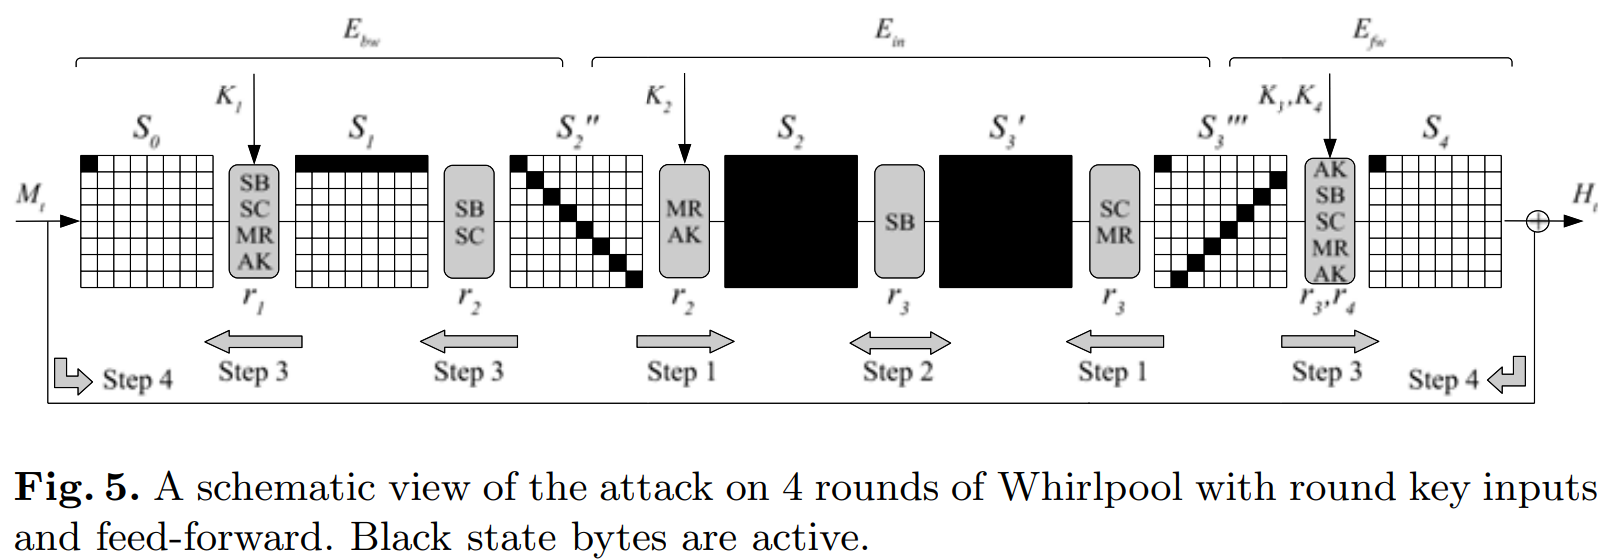
\includegraphics[width=0.75\linewidth]{rebound_view.png}
    \caption{Графическое представление Rebound attack [11]}
    \label{fig:enter-label}
\end{figure}

\subsubsection{Inbound phase. 1 этап}

Выбирается случайная разность с 8 активными байтами состояния (то есть 8 ненулевых байтов, остальные нулевые) $S''_2$ перед слоем MR раунда $r_2$. Все активные байты должны находиться на диагонали состояния $S''_2$ (см. рисунок выше). Затем разности распространяются вперёд до полностью активного состояния на входе следующего слоя SB (состояние $S_2$) с вероятностью 1. Далее мы выбираем другую случайную разность с 8 активными байтами в состоянии $S'''_3$ после функции MR раунда $r_3$ и распространяем её назад. Снова диагональная форма гарантирует, что мы получаем полностью активное состояние на выходе SB раунда $r_3$.

\subsubsection{Inbound phase. 2 этап}

Это шаг, который реализует "встречу посередине". Мы ищем совпадающую входную и выходную разность (вероятный дифференциал) для слоя SB раунда $r_3$, используя заранее вычисленную таблицу дифференциалов S-бокса. Поскольку вероятность нахождения совпадения для каждого байта составляет 1/2, вероятность нахождения дифференциала для всего активного слоя SubBytes составляет примерно $2^{-64}$. Таким образом, после повторения шага 1 атаки примерно $2^{64}$ раз мы ожидаем найти дифференциал SubBytes для всего состояния (все 64 байта одновременно имеют дифференциал). Мы получаем как минимум два значения состояния (слева и справа от SB) для каждого совпадения S-бокса, у нас будет около $2^{64}$ начальных точек для выходного этапа. Эти $2^{64}$ начальных точек можно сконструировать с общей сложностью около $2^{64}$.

\subsubsection{Outbound phase. 3 этап}
В outbound phase мы продолжаем расширять дифференциальную последовательность назад и вперёд. Продвигая вероятный дифференциал слева через следующий слой SubBytes, мы получаем усечённый дифференциал с 8 активными байтами в каждом направлении. Затем усечённые дифференциалы должны распространяться от 8 до 1 активного байта через преобразование MR, как в обратном, так и в прямом направлении.

В [11] показано что, для преобразования 8 активных байтов в 1 активный байт при прохождении через MR в среднем необходимо перебрать $2^{56}$ начальных точек ($2^{7*8}$, где $2^8$ - обратная вероятность появления нулевого значения и 7 их количество). Так как, нужно пройти в 2 направления, то необходимо перебрать $2^{56*2}=2^{112}$ начальных точек. У нас есть необходимое количество попыток, так как в indound фазе мы можем перебирать до $2^{128}$ точек.

\subsubsection{Outbound phase. 4 этап}
Осталось 2 активных байтов по краям и необходимо, чтобы они были одинаковыми чтобы разность на входе и на выходе стали одинаковыми. Вероятность появления одинаковых байтов равна $2*{-8}$. Поэтому необходимо $2^8$ раз повторить последний этап. Итого сложность атаки получилась $2^{112+8}=2^{120}$ операции Whirlpool. Требуемые объем памяти - $2^{16}$. Заметим, что подмешивание ключей влияния не оказывает. Также атака работает со стандартным $IV$. Авторы отмечают, что можно добавить еще полраунда $SB, SC$, так как они не ломают построенный дифференциал. По факту атака проводится над 4 раундами, но получается, что можно добавить еще пару функции и выйдет 4.5 раунда.

\subsubsection{Rebound атака на 5.5 раундов}

Rebound атака на 5.5 раундов выглядит так:

\begin{figure}[H]
    \centering
    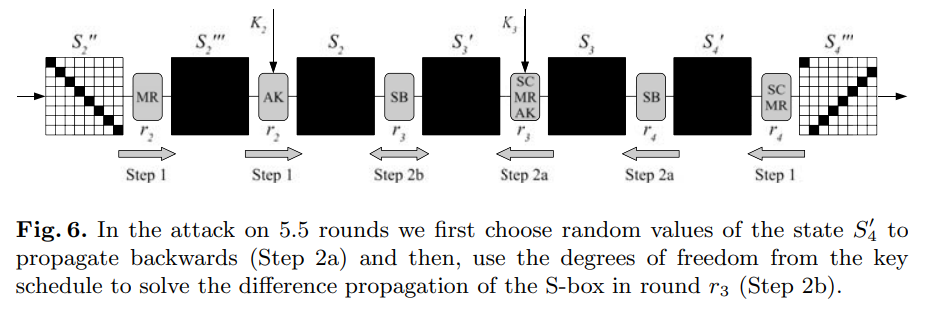
\includegraphics[width=0.75\linewidth]{att_2.png}
    \caption{Rebound атака на 5.5 раундов [11]}
    \label{fig:enter-label}
\end{figure}

Количество операции - $2^{120}$, количество памяти - $2^{16}$.

\subsubsection{Rebound атака на 7.5 раундов}

Rebound атака на 7.5 раундов выглядит так:

\begin{figure}[H]
    \centering
    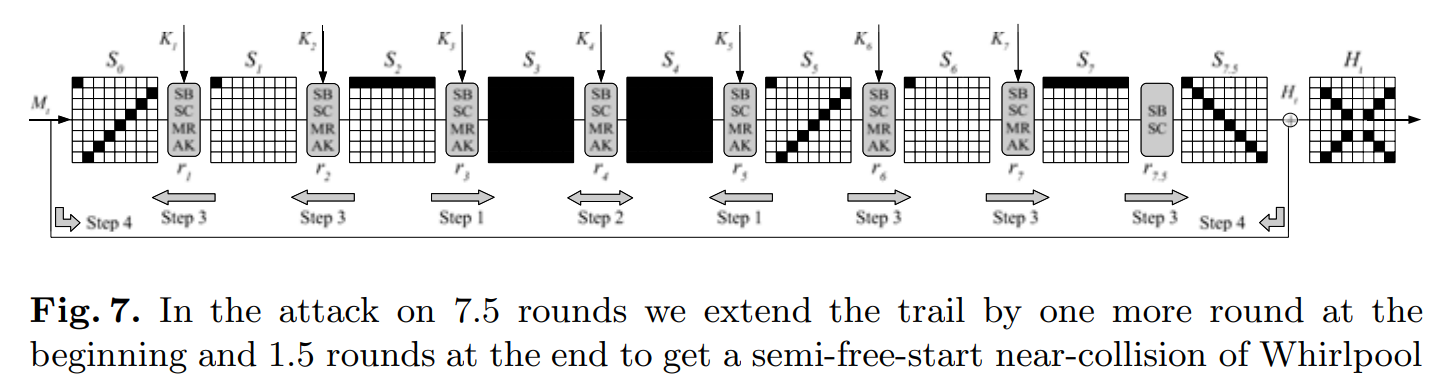
\includegraphics[width=0.75\linewidth]{att_3.png}
    \caption{Rebound атака на 7.5 раундов [11]}
    \label{fig:enter-label}
\end{figure}

Количество операции - $2^{128}$, количество памяти - $2^{16}$.

\subsubsection{Вывод}

Таким образом, эти атаки не представляют практической угрозы нахождения коллизии, так как требуют много операции и работают лишь на определенном количестве раундов. Однако rebound атака имеет значительное теоретическое значение, так как открыло новый вектор исследования криптографических схем.

\subsection{Заключение}

Хеш-функция Whirlpool, основанная на конструкции Меркла-Дамгарда и использующая блочный шифр, на протяжении восьми лет оставалась устойчивой к атакам. Однако в 2009 году была предложена новая атака — Rebound attack, которая позволила находить коллизии на частичных раундах Whirlpool.


\section{Fast Syndrome Based Hash (FSB)}
FSB (Fast Syndrome-Based Hash Function) — это семейство криптографических хеш-функций [12], которое разработали в 2003 году.

FSB использует конструкцию Меркла-Дамгарда с классическим паддингом. Опишем функцию сжатия $f$.

$\newline$

\textbf{Функция сжатия $f$}

На вход эта функция принимает блок длиной $s$, который состоит из предыдущего значения $h$ ($|h|$ = $r$) и блока сообщения $m$ ($|m| = s - r$). Внутри себя она использует булеву матрицу $\mathcal{H}$ размера $r * n$, которая сгенерирована из равномерного распределения над всеми булевыми матрицами соответствующего размера. Должно соблюдаться следующее:

\begin{enumerate}
    \item $n, r, w, s, log_2(n/w)$ должны быть натуральными числами
    \item $s = w*log_2(n/w)$
    \item $s > r$
\end{enumerate}

Матрица $\mathcal{H}$ разбивается на $w$ подматриц $\mathcal{H_i}$ размера $r*(n/w)$. Затем происходит основной алгоритм:

\begin{enumerate}
    \item Входной блок $s$ разбивается на $w$ подряд идущих векторов, каждый из которых отображается в то неотрицательное число, двоичной записью которого этот вектор является. Таким образом $s$ переходит в $(s_1, \ldots, s_w)$.
    \item Далее из каждой подматрицы $\mathcal{H_i}$ выбирается $s_i$ столбец. Затем эти столбцы складываются по модулю 2 и сохраняется в переменную $h$.
    \item На выход подается $h$, длина $h$ равна $r$.
\end{enumerate}

\section{Список литературы}
[1] Миронкин В. О. Об одной теоретико-вероятностной модели Sponge-конструкции //Обозрение прикладной и промышленной математики. – 2018. – Т. 25. – №. 1. – С. 3-8.

[2] Rivest R. The MD5 message-digest algorithm. – 1992. – №. rfc1321.

[3] Standard S. H. Secure hash standard //FIPS PUB. – 1995. – С. 180-1.

[4] Eastlake 3rd D., Jones P. US secure hash algorithm 1 (SHA1). – 2001. – №. rfc3174.

[5] Secure hash standard //FIPS PUB 180-2. – 2002.

[6] ГОСТ 28147-89 на сайте ФГУП «Стандартинформ» // URL: https://www.gostinfo.ru/catalog/Details/?id=4149371

[7] Kazymyrov O., Kazymyrova V. Algebraic aspects of the russian hash standard GOST R 34.11-2012 //Cryptology ePrint Archive. – 2013.

[8] ГОСТ 34.11-2018 «Информационная технология. Криптографическая защита информации. Функция хэширования» // URL: http://protect.gost.ru/v.aspx?control=7&id=232143

[9] Block-diagram of BLAKE hash function algorythm // URL: https://commons.wikimedia.org/wiki/File:BLAKE_algorythm.png

[10] Aumasson J. P. et al. Sha-3 proposal blake //Submission to NIST. – 2008. – Т. 92. – С. 194.

[11] Barreto P. et al. The Whirlpool hashing function //First open NESSIE Workshop, Leuven, Belgium. – 2000. – Т. 13. – С. 14.

[12] Augot D., Finiasz M., Sendrier N. A fast provably secure cryptographic hash function //Cryptology ePrint Archive. – 2003.

[13] Mendel F. et al. The rebound attack: Cryptanalysis of reduced Whirlpool and Grøstl //Fast Software Encryption: 16th International Workshop, FSE 2009 Leuven, Belgium, February 22-25, 2009 Revised Selected Papers. – Springer Berlin Heidelberg, 2009. – С. 260-276.

\end{document}
